% Options for packages loaded elsewhere
\PassOptionsToPackage{unicode}{hyperref}
\PassOptionsToPackage{hyphens}{url}
%
\documentclass[
]{article}
\usepackage{lmodern}
\usepackage{amssymb,amsmath}
\usepackage{ifxetex,ifluatex}
\ifnum 0\ifxetex 1\fi\ifluatex 1\fi=0 % if pdftex
  \usepackage[T1]{fontenc}
  \usepackage[utf8]{inputenc}
  \usepackage{textcomp} % provide euro and other symbols
\else % if luatex or xetex
  \usepackage{unicode-math}
  \defaultfontfeatures{Scale=MatchLowercase}
  \defaultfontfeatures[\rmfamily]{Ligatures=TeX,Scale=1}
\fi
% Use upquote if available, for straight quotes in verbatim environments
\IfFileExists{upquote.sty}{\usepackage{upquote}}{}
\IfFileExists{microtype.sty}{% use microtype if available
  \usepackage[]{microtype}
  \UseMicrotypeSet[protrusion]{basicmath} % disable protrusion for tt fonts
}{}
\makeatletter
\@ifundefined{KOMAClassName}{% if non-KOMA class
  \IfFileExists{parskip.sty}{%
    \usepackage{parskip}
  }{% else
    \setlength{\parindent}{0pt}
    \setlength{\parskip}{6pt plus 2pt minus 1pt}}
}{% if KOMA class
  \KOMAoptions{parskip=half}}
\makeatother
\usepackage{xcolor}
\IfFileExists{xurl.sty}{\usepackage{xurl}}{} % add URL line breaks if available
\IfFileExists{bookmark.sty}{\usepackage{bookmark}}{\usepackage{hyperref}}
\hypersetup{
  pdftitle={Fieldsurvey},
  hidelinks,
  pdfcreator={LaTeX via pandoc}}
\urlstyle{same} % disable monospaced font for URLs
\usepackage[margin=1in]{geometry}
\usepackage{longtable,booktabs}
% Correct order of tables after \paragraph or \subparagraph
\usepackage{etoolbox}
\makeatletter
\patchcmd\longtable{\par}{\if@noskipsec\mbox{}\fi\par}{}{}
\makeatother
% Allow footnotes in longtable head/foot
\IfFileExists{footnotehyper.sty}{\usepackage{footnotehyper}}{\usepackage{footnote}}
\makesavenoteenv{longtable}
\usepackage{graphicx}
\makeatletter
\def\maxwidth{\ifdim\Gin@nat@width>\linewidth\linewidth\else\Gin@nat@width\fi}
\def\maxheight{\ifdim\Gin@nat@height>\textheight\textheight\else\Gin@nat@height\fi}
\makeatother
% Scale images if necessary, so that they will not overflow the page
% margins by default, and it is still possible to overwrite the defaults
% using explicit options in \includegraphics[width, height, ...]{}
\setkeys{Gin}{width=\maxwidth,height=\maxheight,keepaspectratio}
% Set default figure placement to htbp
\makeatletter
\def\fps@figure{htbp}
\makeatother
\setlength{\emergencystretch}{3em} % prevent overfull lines
\providecommand{\tightlist}{%
  \setlength{\itemsep}{0pt}\setlength{\parskip}{0pt}}
\setcounter{secnumdepth}{5}

\title{Fieldsurvey}
\usepackage{etoolbox}
\makeatletter
\providecommand{\subtitle}[1]{% add subtitle to \maketitle
  \apptocmd{\@title}{\par {\large #1 \par}}{}{}
}
\makeatother
\subtitle{Associations of organic matter quality and soil diversity to long term dieldrin loss}
\author{}
\date{\vspace{-2.5em}}

\begin{document}
\maketitle

{
\setcounter{tocdepth}{2}
\tableofcontents
}
\hypertarget{results}{%
\section{Results}\label{results}}

\hypertarget{carbon-quality}{%
\subsection{Carbon quality}\label{carbon-quality}}

\begin{figure}
\centering
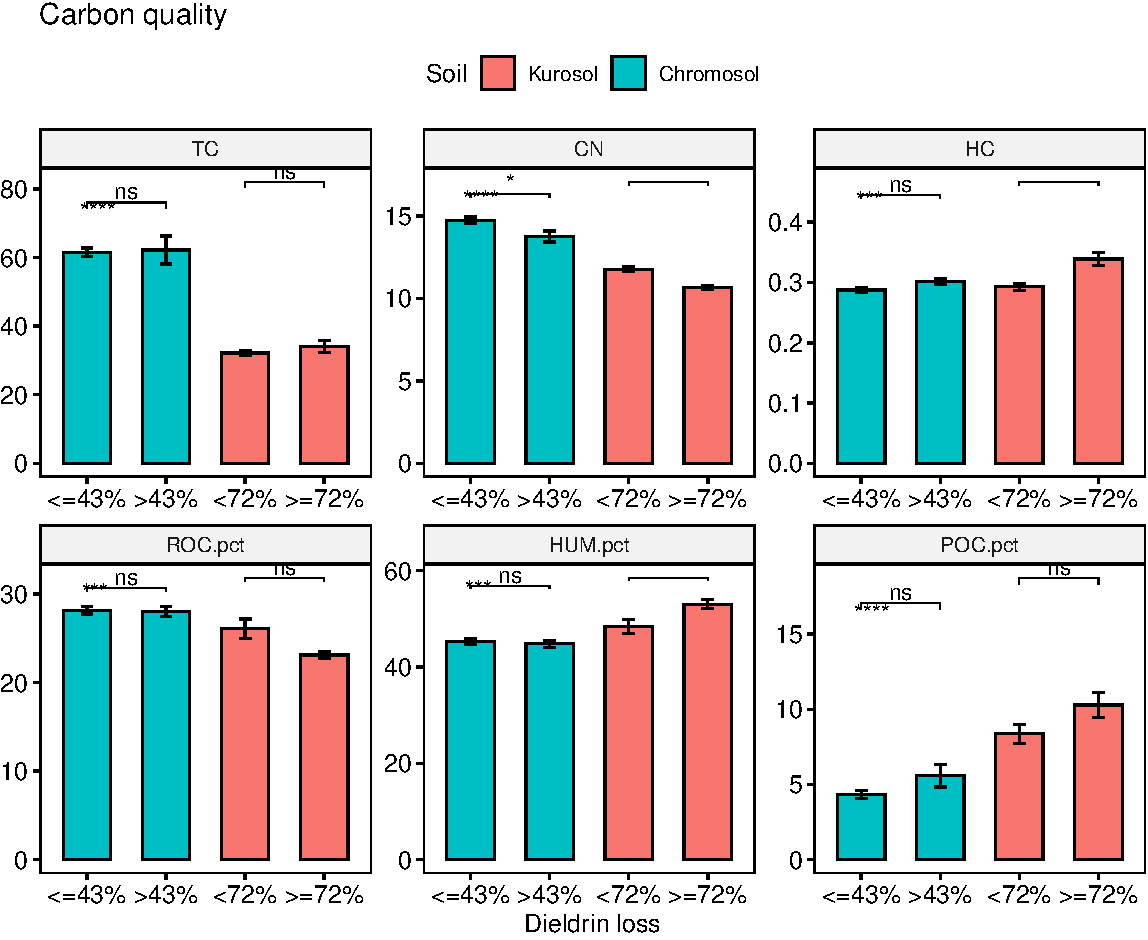
\includegraphics{M2_Results_files/figure-latex/carbonquality-1.pdf}
\caption{\label{fig:carbonquality}Comparisons of carbon quality variables between samples of low and high dieldrin loss. Samples are grouped by long-term dielrin loss (\%) where the loss is either below or above the median loss in each soil type. Significance of global Kruskal-Wallis tests and Wilcoxon tests for each soil type are shown.}
\end{figure}

Overall the two soils contained a different carbon quantity and quality. (Fig. \ref{fig:carbonquality}) shows that the Kursol, the soil with greater long-term dieldrin losses, contained significantly less total carbon (TC). Although it was less rich in organic matter, it was composed of more humus (HUM) and particulate organic carbon (POC) relative to the resistant organic carbon (ROC). Furthermore, a high-loss soil environments coincided with a low carbon-to-nitrogen ration (C:N), and higher hydrogen-to-carbon ration (H:C) and a higher proportion of humus in the Kurosol.
There was also a trend that indicated that a higher proportion of POC was associated with more dieldrin loss.

\hypertarget{alpha-diversity}{%
\subsection{Alpha diversity}\label{alpha-diversity}}

\begin{figure}
\centering
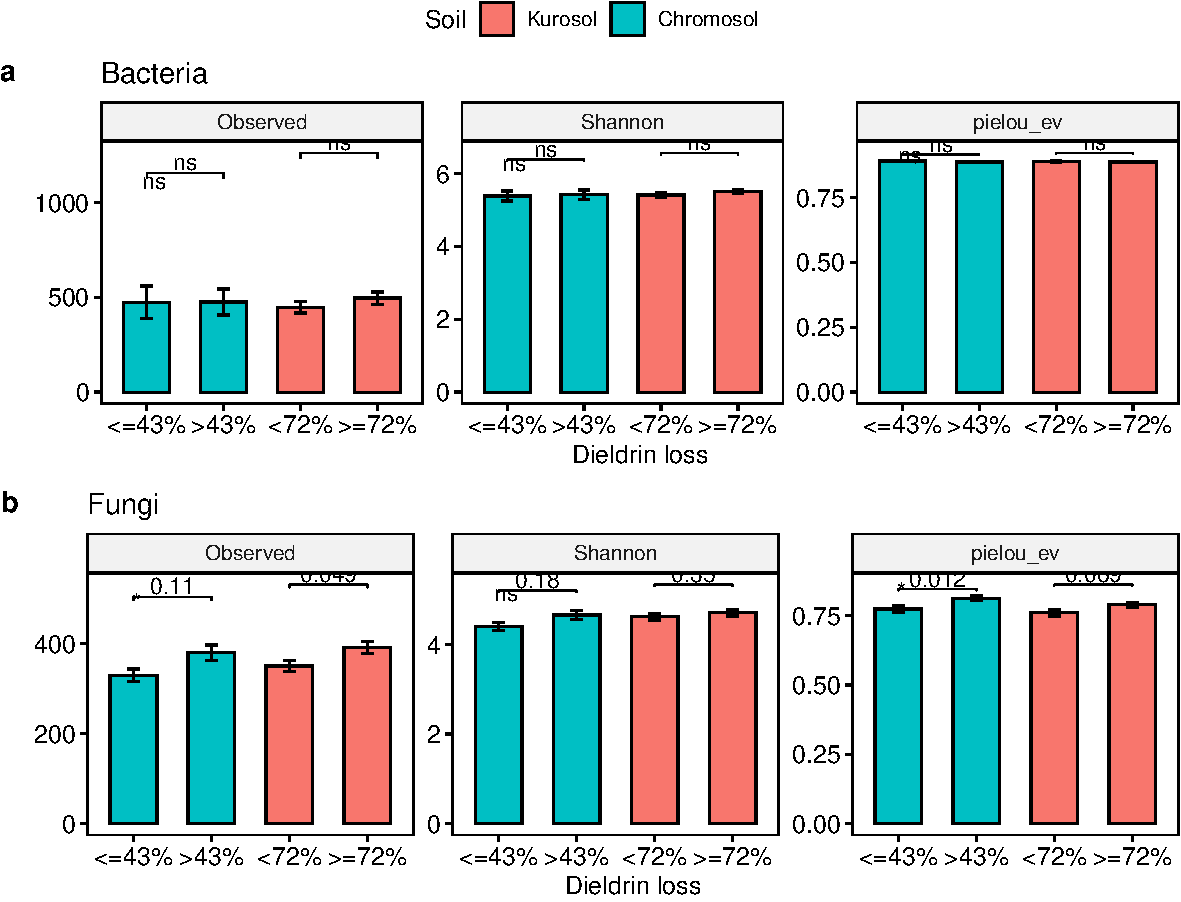
\includegraphics{M2_Results_files/figure-latex/alphadloss-1.pdf}
\caption{\label{fig:alphadloss}Alpha diversity of bacteria and fungi. Samples are grouped by long-term dielrin loss (\%) where the loss is either below or above the median loss in each soil type. Significance of global Kruskal-Wallis tests and Wilcoxon tests for each soil type are shown.}
\end{figure}

Only the fungal alpha diversity was associated with the long-term dieldrin loss (Fig. \ref{fig:alphadloss}b) not the bacterial diversity (Fig. \ref{fig:alphadloss}a). For example, fungal pielou evenness was greater in samples that were associated with high long-term dieldrin loss. Hence in a high-loss environment, the fungal OTUs were distributed more evenely. Furthermore, the mean number of observed fungal OTUs was higher in samples that had high long-term dieldrin loss.

\begin{figure}
\centering
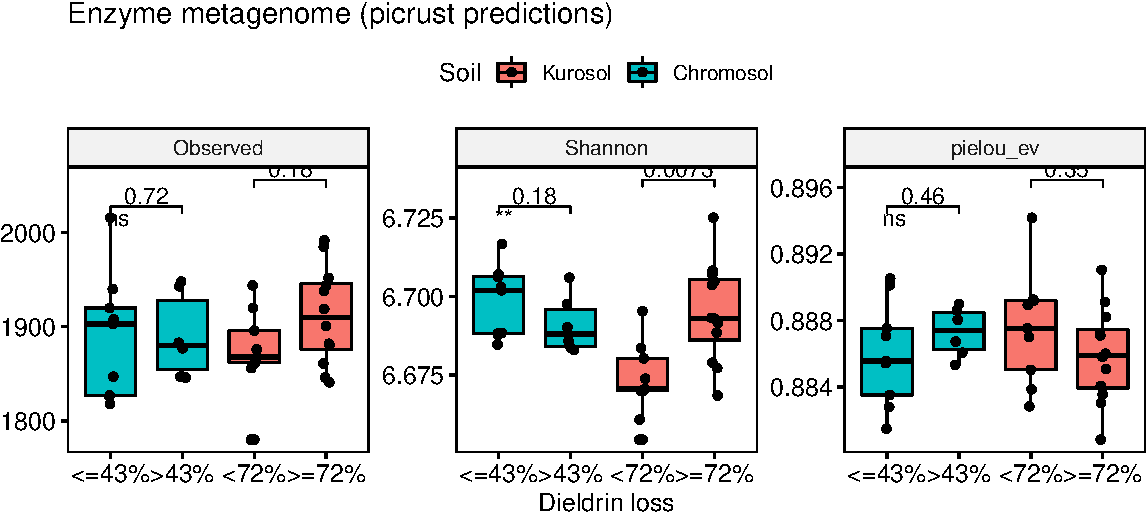
\includegraphics{M2_Results_files/figure-latex/alphadlossenzymes-1.pdf}
\caption{\label{fig:alphadlossenzymes}Alpha diversity of enzyme metagenome as prediced by picrust2. Samples are grouped by long-term dielrin loss (\%) where the loss is either below or above the median loss in each soil type. Significance of global Kruskal-Wallis tests and Wilcoxon tests for each soil type are shown.}
\end{figure}

The functional diversity based on the predicted enzyme metagenome was similar across the two soils (Fig. \ref{fig:alphadlossenzymes}). However, in the Kurosol, the shannon diversity was greater in the high-loss samples while the number of observed enzymes and pilou evenness remained the same. Shannon's index accounts for both abundance and evenness so an increase of this index without an increase in evenness, indicated that more enzyme were with greater abundance were present in the high-loss environment.

\begin{figure}
\centering
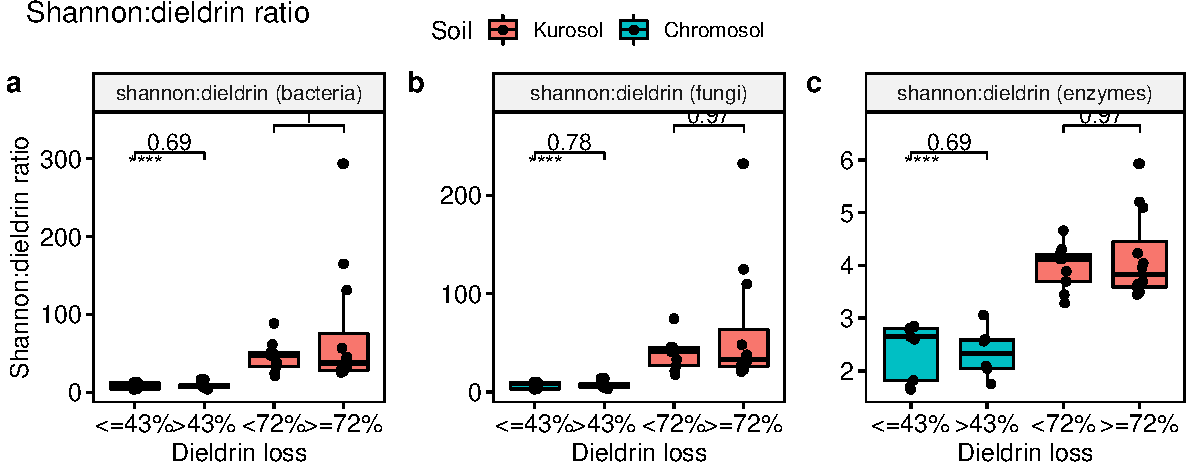
\includegraphics{M2_Results_files/figure-latex/alphaperD17-1.pdf}
\caption{\label{fig:alphaperD17}Shannon:dieldrin ratio to compare diversity per unit dieldrin (µg/g). Samples are grouped by long-term dielrin loss (\%) where the loss is either below or above the median loss in each soil type. Significance of global Kruskal-Wallis tests and Wilcoxon tests for each soil type are shown.}
\end{figure}

Soil diversity per unit dieldrin (µg/g) was compared (Fig \ref{fig:alphaperD17}). It showed that the Kurosol, which contained less organic matter and dieldrin, had significantly higher diversity for each µg/g of dieldrin compared to the Kurosol. Hence, there was greater diversity for each molecule of dieldrin in the high-loss environment.

\hypertarget{metabolic-potential}{%
\subsection{Metabolic potential}\label{metabolic-potential}}

\begin{figure}
\centering
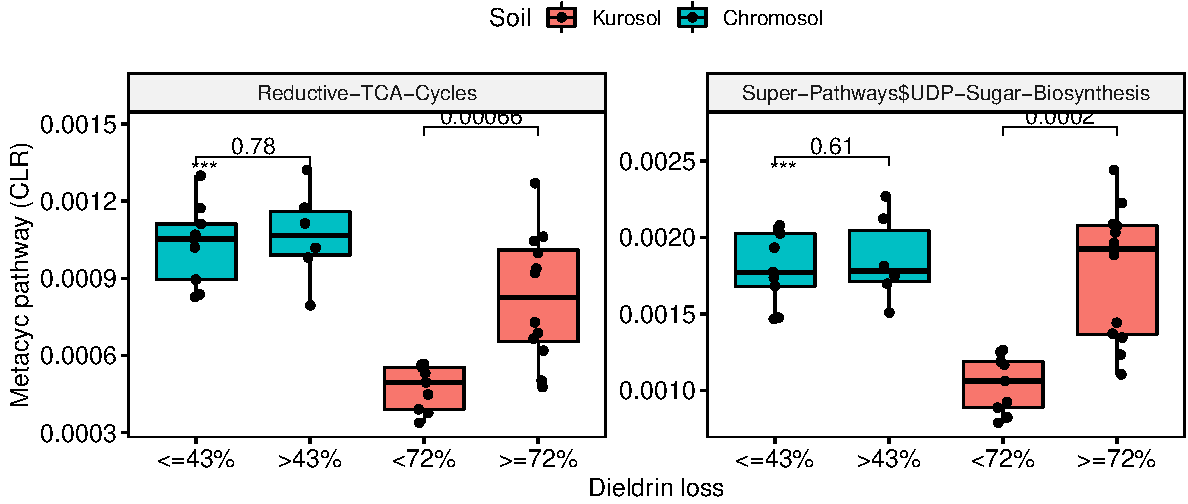
\includegraphics{M2_Results_files/figure-latex/plsdakur-1.pdf}
\caption{\label{fig:plsdakur}Kurosol: Potentials of metabolic pathways which were predicted to be different between samples with low and high dieldrin loss (\%) by partial least squares discriminant anaylysis (PLS-DA). Samples are grouped by long-term dielrin loss (\%) where the loss is either below or above the median loss in each soil type. Significance of global Kruskal-Wallis tests and Wilcoxon tests for each soil type are shown.}
\end{figure}

(Fig \ref{fig:plsdakur})

\begin{figure}
\centering
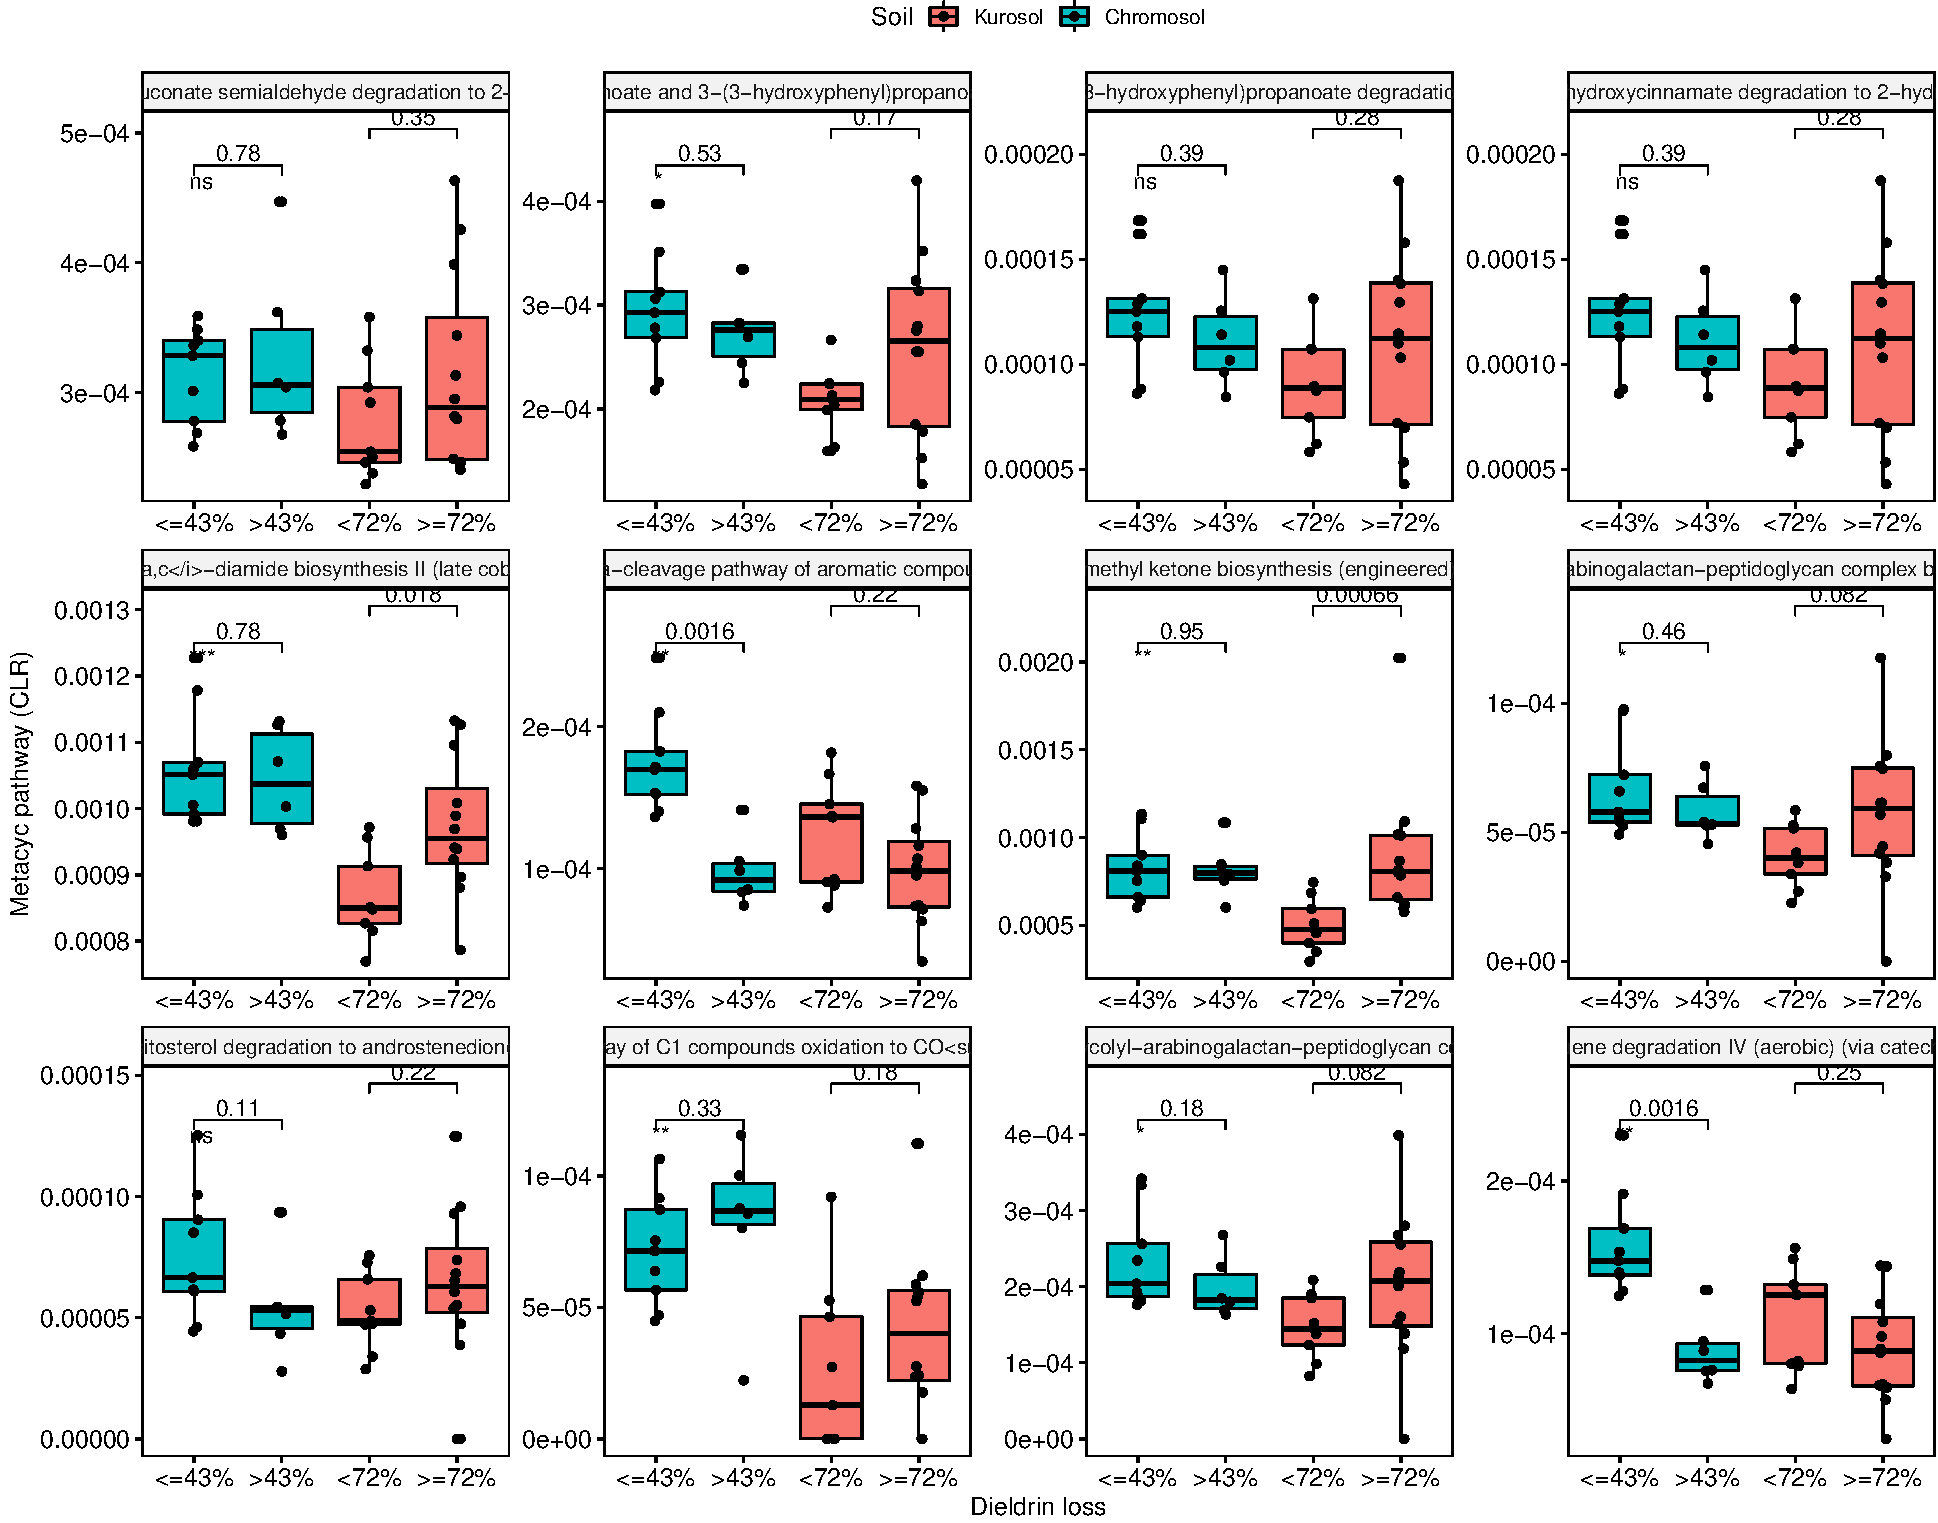
\includegraphics{M2_Results_files/figure-latex/plsdach-1.pdf}
\caption{\label{fig:plsdach}Chromosol: Potentials of metabolic pathways which were predicted to be different between samples with low and high dieldrin loss (\%) by partial least squares discriminant anaylysis (PLS-DA). Samples are grouped by long-term dielrin loss (\%) where the loss is either below or above the median loss in each soil type. Significance of global Kruskal-Wallis tests and Wilcoxon tests for each soil type are shown.}
\end{figure}

(Fig \ref{fig:plsdach})

\begin{figure}
\centering
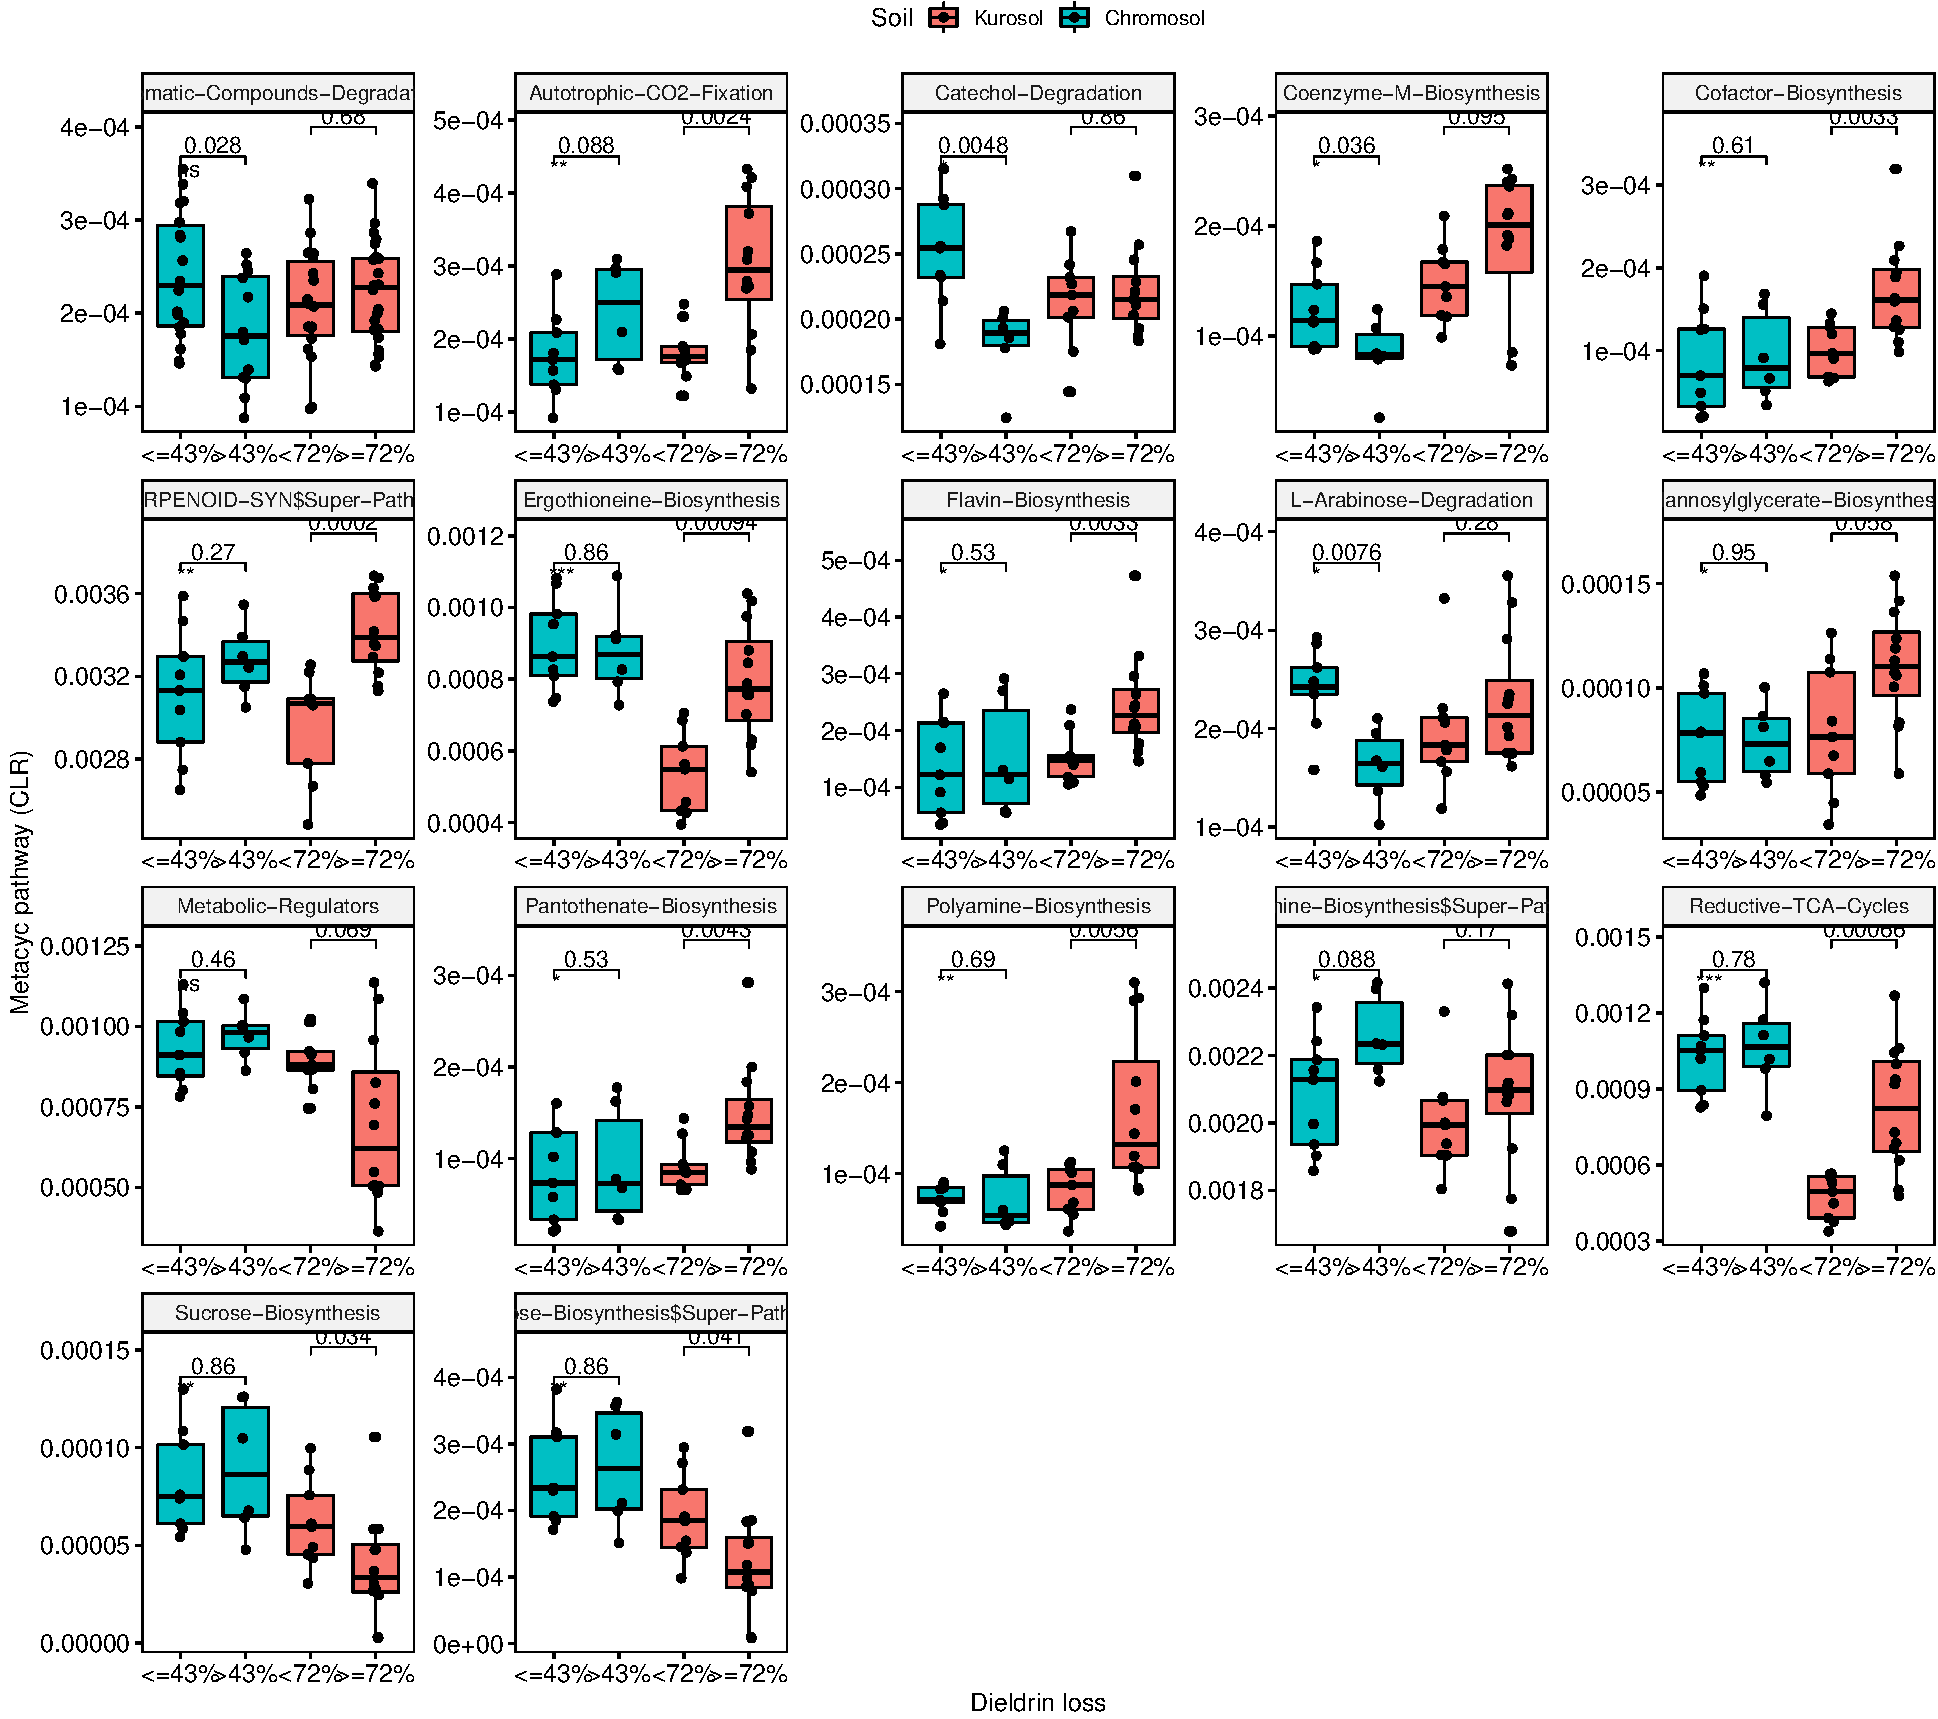
\includegraphics{M2_Results_files/figure-latex/plsda_all-1.pdf}
\caption{(\#fig:plsda\_all)Across all 36 samples: Potentials of metabolic pathways which were predicted to be different between samples with low and high dieldrin loss (\%) by partial least squares discriminant anaylysis (PLS-DA). Samples are grouped by long-term dielrin loss (\%) where the loss is either below or above the median loss in each soil type. Significance of global Kruskal-Wallis tests and Wilcoxon tests for each soil type are shown.}
\end{figure}

(Fig @ref(fig:plsda\_all))

\hypertarget{betadiversity}{%
\subsection{Betadiversity}\label{betadiversity}}

\hypertarget{pcoa-and-nmds}{%
\subsubsection{pcoa and nmds}\label{pcoa-and-nmds}}

\begin{figure}
\centering
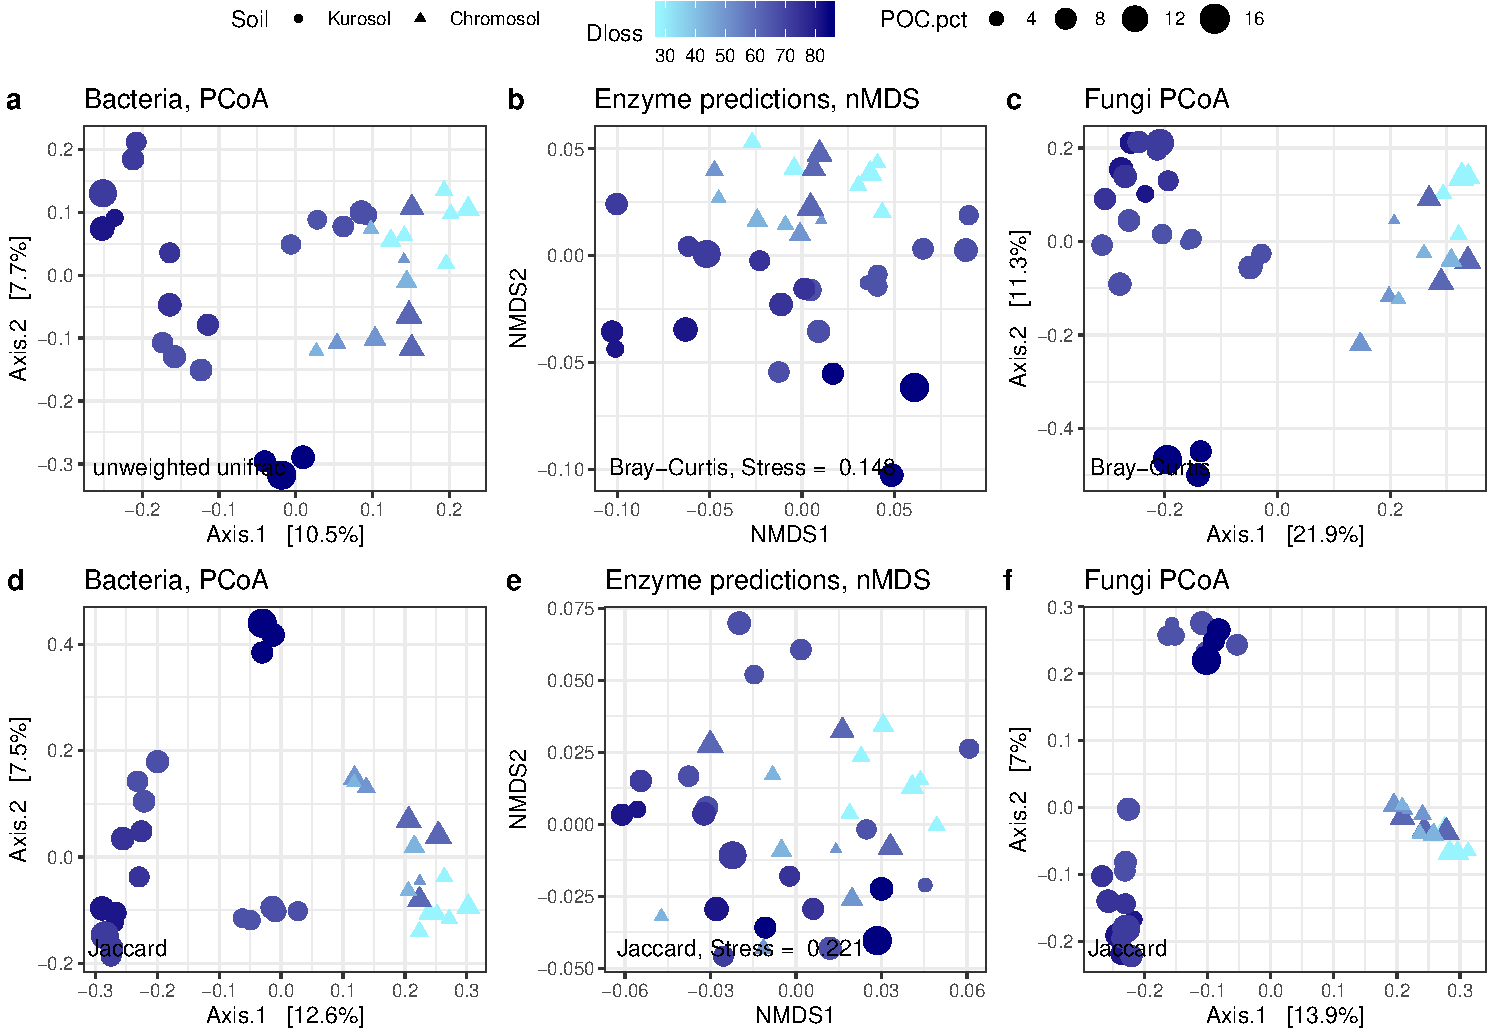
\includegraphics{M2_Results_files/figure-latex/pcoa-1.pdf}
\caption{\label{fig:pcoa}Ordinations of two different dissimilarity indices are compared for each composition of bacteria, their enzyme predictions and fungi.}
\end{figure}

(Fig. \ref{fig:pcoa})

\begin{itemize}
\tightlist
\item
  Bacteria (a \& d)

  \begin{itemize}
  \tightlist
  \item
    Bacterial compositional comparison was made between a phylogenetic presence and absence distances metric (unweighted unifrac) and a non-phylogenetic presence and absence distance metric (Jaccard).
  \item
    Overall, a greater community dispersion was seen in the Kurosol. Phylogeny from the unifrac metric did not make a difference to this community dispersion in the Kurosol so the differences in OTU composition also infer genetic dispersion.
  \item
    This is in contrast to the Chromosol, which contained a more homogenous pool of OTUs
  \end{itemize}
\item
  Enzyme metagenome (functional potential of bacteria) (b \& e)

  \begin{itemize}
  \tightlist
  \item
    Bray-Curtis (abundance) was compared to Jaccard distance (presence absence)
  \item
    There were similar genes present in each soil but their estimated abundances differed.
  \item
    While a higher dispersion of gene abundances was observed in the Kurosol, the gene abundances in the Chromosol were homogenous. This meant that the metabolic potentials were more differentially abundant in the soil with high dieldrin loss.
  \end{itemize}
\end{itemize}

\hypertarget{rda}{%
\subsubsection{rda}\label{rda}}

\begin{figure}
\centering
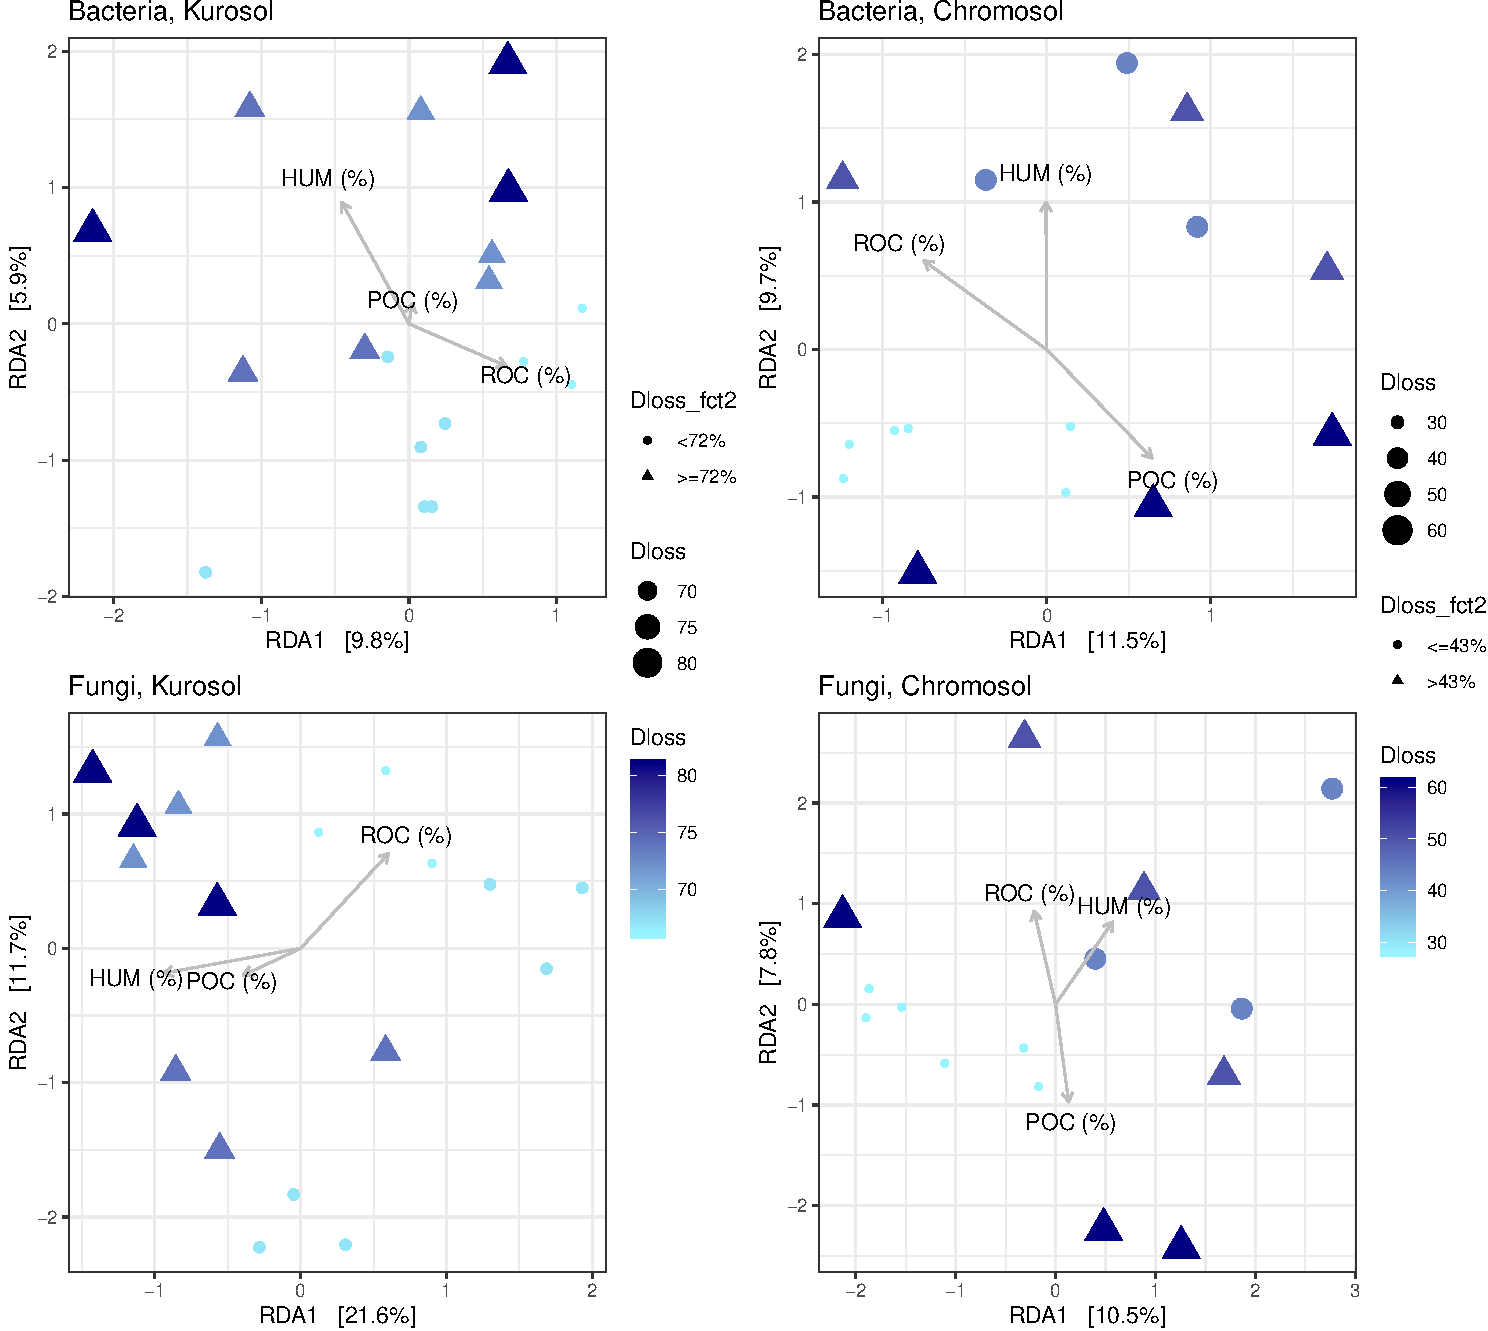
\includegraphics{M2_Results_files/figure-latex/rda-1.pdf}
\caption{\label{fig:rda}Ordinations of two different dissimilarity indices are compared for each composition of bacteria, their enzyme predictions and fungi.}
\end{figure}

\hypertarget{pls}{%
\subsubsection{pls}\label{pls}}

\begin{figure}
\centering
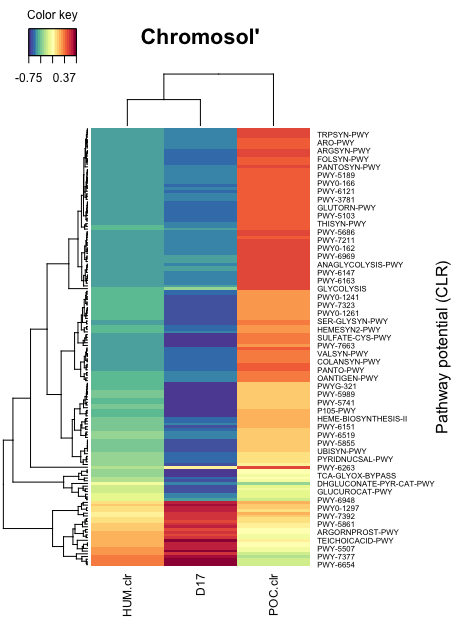
\includegraphics{./Images/correlationheatmap_mixomix_pls_ch_canonical_2axis_20feb_threshold0.5_scaled.png}
\caption{\label{fig:plsheatmapsch}Partial least squares analysis in canonical mode for Chromosol samples}
\end{figure}

(Fig \ref{fig:plsheatmapsch})

\begin{figure}
\centering
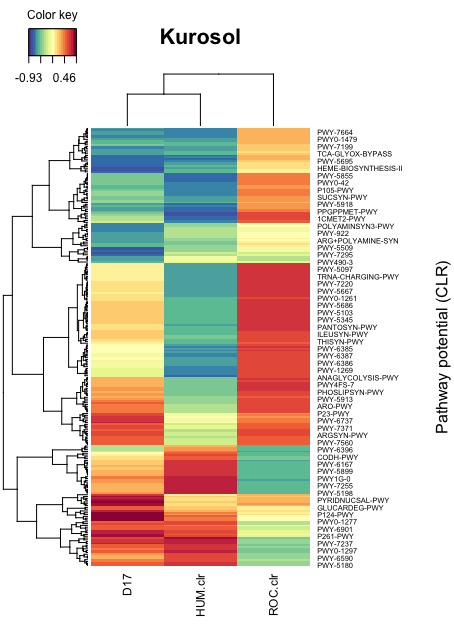
\includegraphics{./Images/correlationheatmap_mixomix_pls_ku_canonical_2axis_20feb_threshold0.5_scaled.png}
\caption{\label{fig:plsheatmapsku}test}
\end{figure}

(Fig \ref{fig:plsheatmapsku})

\end{document}
